\addtocontents{toc}{\setcounter{tocdepth}{3}}
\chapter{Analyse et spécification des besoins}

\section*{Introduction}
Dans ce chapitre, nous allons identifier les besoins fonctionnels et les besoins non fonctionnels de notre système ainsi que nous allons  présenter le diagramme de cas d’utilisation global en utilisant UML. Nous allons établir ensuite le Backlog Produit et la planification des sprints.

% Une section
\section{Analyse des besoins}

Dans cette section, nous allons identifier les acteurs de notre système, exposer les besoins fonctionnels et les besoins non fonctionnels de notre application.
\subsection{ Identification des acteurs}
Un acteur est une entité externe au système. Il représente une personne ou un autre système informatique qui attend un ou plusieurs services offerts par une interface d’accès. Il interagit avec le système par envoi ou réception des messages \cite{identificationActeur}.\\
Les acteurs qui interagissent avec l’application sont de deux types :
       \begin{itemize}
    \item Administrateur : c'est la personne possédant le privilège de plus haut niveau et il a l'accès à toutes les fonctionnalités du notre application. Il permet aussi de gérer les différents utilisateurs.
    \item Utilisateur de ressource humaine : chaque utilisateur de ressource humaine a le droit de gérer les informations des employés de Sofrecom, d'effectuer des prédictions et de consulter le tableau de bord.
 \end{itemize}
    \subsection{Besoins fonctionnels}
      Il s’agit principalement des fonctionnalités offertes par l’application aux utilisateurs. Ces besoins expriment une action devant être effectuée par l’application en réponse à une demande. Cette application offre les fonctionnalités suivantes :
   
       \begin{itemize}
    \item Créer un modèle de prédiction;
    \item S'authentifier;
    \item Gérer les employés;
     \item Importer les données des employés;
      \item Gérer les prédictions;
      \item Consulter l'historique des prédictions effectuées;
      \item Consulter le tableau de bord;
      


      
    \end{itemize}
    Nous allons dans ce stade détailler le contenu des fonctionnalités importantes de notre système.
       
       \begin{itemize}
    \item Créer un modèle de prédiction : \\
    Le processus de création d'un modèle de prédiction implique de fournir un algorithme d'apprentissage qui permet de trouver des dépendances et des patterns entre des données nommées données d'entraînement.
    
    Les données d'entraînement doivent contenir la bonne réponse, connue sous le nom de cible ou d'attribut cible. L'algorithme d'apprentissage trouve des règles dans les données d'entraînement qui mettent en correspondance les attributs des données d'entrée avec la cible (la variable de prédiction) et il produit un modèle qui capture ces patterns.\\
    Nos données concernent les informations des employés de Sofrecom (matricule, civilité, âge, expérience de travail avant sofrecom,expérience de travail dans sofrecom, expérience de travail totale, poste, pôle, manager, situation familiale, séniorité) et la cible concerne la démission des employés ( « 1 » : l'employé va démissionner,   « 0 » : l’employé va rester dans Sofrecom  ).\\ Nous allons  créer un modèle pour obtenir des prédictions sur de nouvelles données pour lesquelles nous ne connaissons pas la cible. Notre modèle devra etre capable d'effectuer des prédictions sur la sortie des employés.
  \\
   \item Gérer les prédictions : \\
 Après la création du modèle, l'utilisateur peut effectuer une prédiction sur la démission d'un employé existant ou un nouveau employé. Il peut aussi consulter et supprimer des prédictions effectuées.
  \\
   \item Gérer les employés : \\
  L'utilisateur peut gérer les informations concernant les employés (civilité, âge, expérience de travail dans sofrecom, poste, pôle, manager...). L’utilisateur peut ajouter un nouvel employé,
modifier les informations concernant un l'employé, supprimer ou rechercher un employé et consulter la liste des employés.
      \\
      \newpage
         \item Consulter le tableau de bord : \\
Un tableau de bord est un échantillon réduit d'indicateurs permettant à l’utilisateur de suivre l'évolution des résultats et les écarts par rapport à des valeurs de référence. Il permet, aussi, d’évaluer la performance, de réaliser un diagnostic de la situation et de progresser de façon continue.
\\
Le tableau de bord de notre application offre plusieurs indicateurs au niveau de suivi des employés : 

 \begin{itemize}[label=\textbullet]
        \item Classés selon (civilité, manager, situation familiale...);
        \item Nombre de prédiction par date;
        \item Estimation de nombre de démissions par date.
     \end{itemize}
             \end{itemize}
    % Une deuxième sous section
    \subsection{Besoins non fonctionnels}
Ces besoins correspondent aux caractéristiques de l’application, ils permettent d’identifier les contraintes internes et externes du domaine étudié.
L'application a les exigences non fonctionnelles suivantes :\\
\textbf{a) Sécurité }\\
La sécurité permet de définir les niveaux d’accès possibles à l’application. Un utilisateur non authentifié ne possède pas le droit d’accéder à l’application. Seuls les utilisateurs qui ont été créés par l’administrateur ont les droits d’accéder.\\
\textbf{b)	Ergonomie }\\
L’application doit offrir une interface conviviale et facile à utiliser.\\
\textbf{c) Portabilité et compatibilité }\\
L’application doit être portable sur tous les environnements logiciels (Windows, Mac OS, Linux...) et compatible avec tous les navigateurs.\\
\textbf{d) Maintenabilité }\\
L’architecture doit permettre l’évolution et assurer l’extensibilité de l’application.\\
\textbf{d) Performance }\\
Les performances d’exécution de l’application sont, généralement, décrits en termes de (temps de réponse, espace mémoire nécessaire, nombre d’utilisateurs…).
Notre application doit avoir un temps minimal pour rendre une vue dans le navigateur.
%\textbf{c) La performance :}\\%
%Les performances d’exécution de l’application sont, généralement, décrits en termes de (temps de réponse, espace de stockage, nombre d’utilisateurs…).%
% Une deuxième section

\section{Diagramme des cas d'utilisation global}

     Le cas d’utilisation décrit l’action offerte par l’application en réponse à la demande d’un utilisateur.
     Le diagramme de cas d’utilisation représente les fonctionnalités définies et les interactions entre les utilisateurs et l’application \cite{usecaseUml}.
   
       Le diagramme de cas d'utilisation ci-après expose les différents besoins généraux, qui seront détaillés par la suite.
      \begin{figure}[htpb]
\centering
%\fcolorbox{brown}{white}{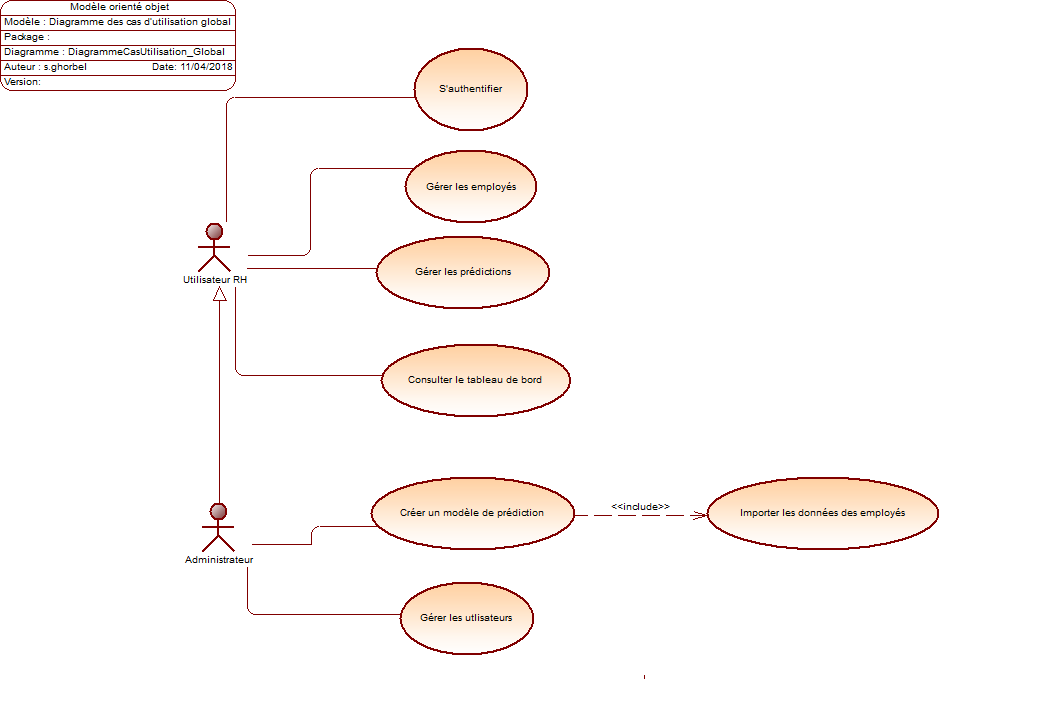
\includegraphics[width=1\linewidth]{img/usecaseglobal_final4.png}}
\fcolorbox{brown}{white}{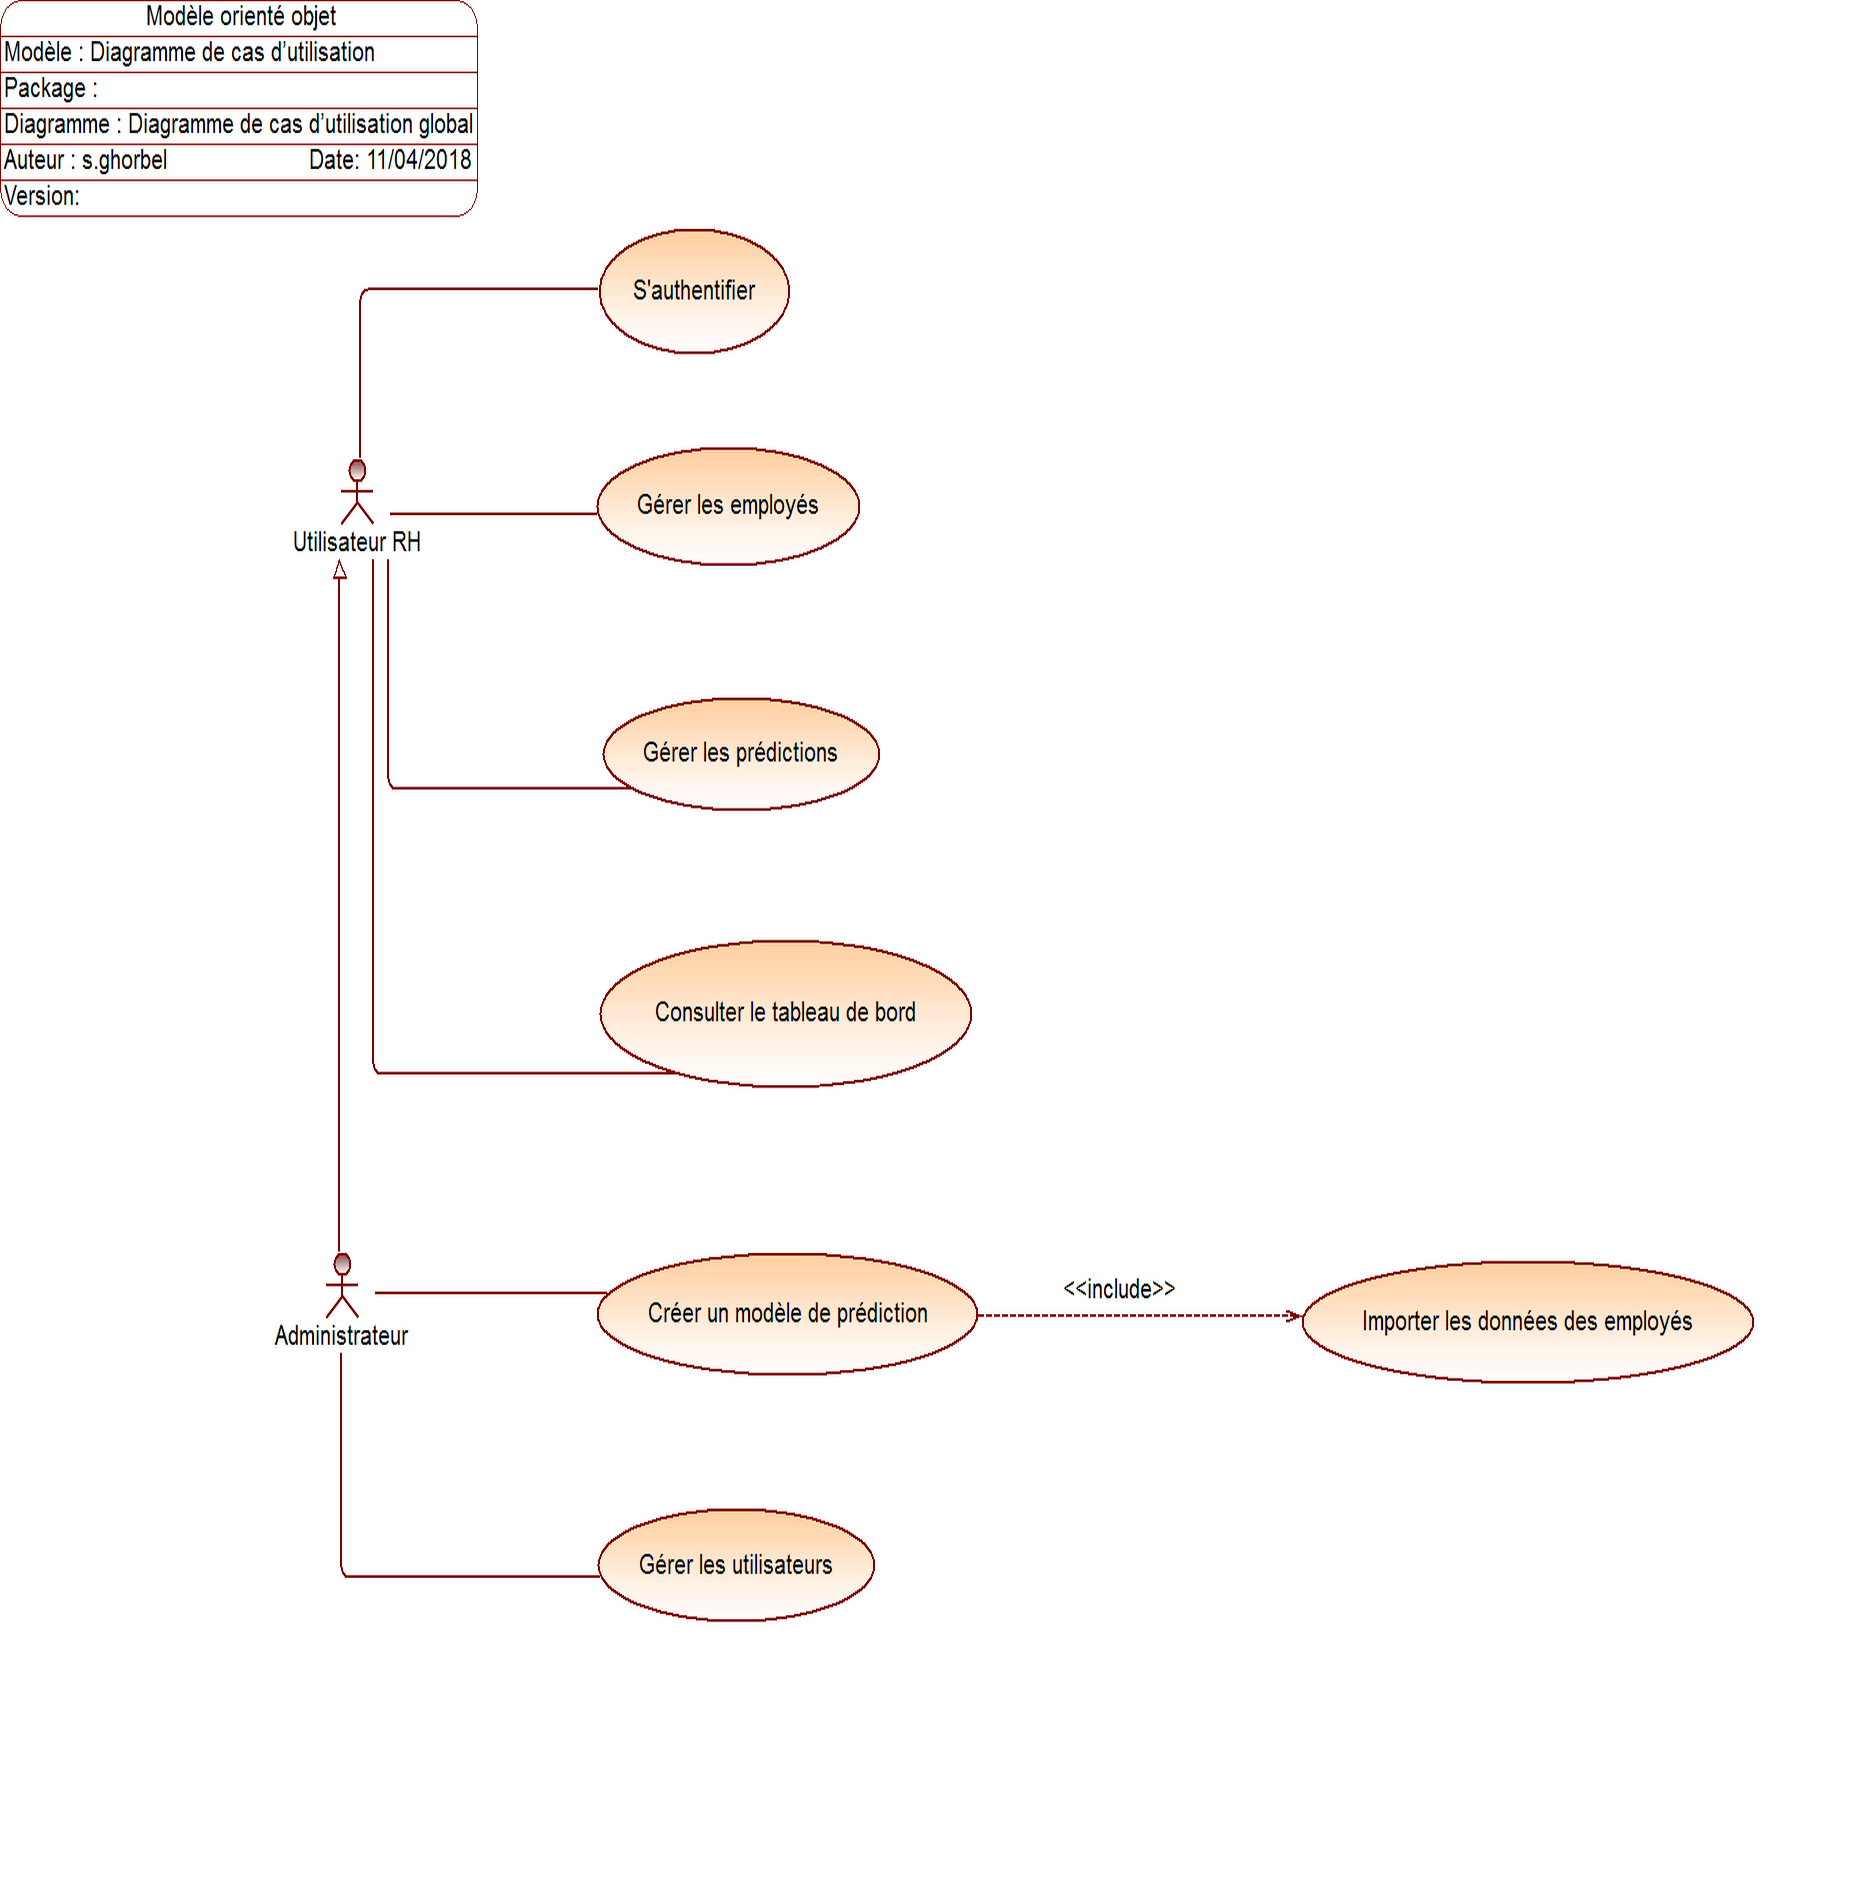
\includegraphics[width=1\linewidth]{img/usecaseglobal_final5_final6.png}}
\caption{Diagramme de cas d'utilisation global}
\label{fig:Diagrammedecasd'utilisationgénéral}
\end{figure}
 


\newpage



     \section{Backlog du produit}
Le tableau 2.1 représente le backlog du produit. Ce tableau est une liste ordonnée qui fournit les éléments suivants
, qui sont traduits dans celui-ci par des "user story" dont: 
 \begin{itemize}
\item ID  représente l’identifiant du user story ;
\item Scénario ou User Story : décrit un comportement du produit visible pour les utilisateurs et
qui leur apporte de la valeur ou de l’utilité ;
\item Priorité de user story est affectée selon la valeur métier et l’ordre de réalisation, où le
chiffre\newline « l » désigne la priorité la plus élevée, « 2 » désigne la priorité élevée, « 3 » désigne la priorité normale ;
\item Pour estimer la complexité de nos user story, nous les avons notées par A pour normal, B pour difficile, C pour dur et D pour très dur.

\end {itemize}

\captionof{table}{Backlog du produit}

\begin{tabular}{@{}| >{\centering\arraybackslash}p{.04\textwidth}| >{\centering\arraybackslash}p{.25\textwidth}|p{6 cm}| >{\centering\arraybackslash}p{.10\textwidth}| >{\centering\arraybackslash}p{.13\textwidth}|@{}}

\hline \rowcolor{lightgray} \textbf{ID}  &  \textbf {Fonctionnalité} & \hspace{1.5pc}  \textbf {Scénario ou User Story} &   \textbf {Priorité} &  \textbf{Complexité} \\

\hline  1 & Création du modèle de prédiction. & En tant qu’administrateur, je veux importer un fichier contenant toutes les informations des employés. & 1 & C \\

\hline  2 &Création du modèle de prédiction.& En tant qu’administrateur, je veux préparer mes données. & 1 & D \\



\hline  3 &Création du modèle de prédiction.& En tant qu’administrateur, je veux construire un modèle de prédiction.& 1 & D \\

\hline  4 &Création du modèle de prédiction.& En tant qu’administrateur, je souhaite évaluer mon modèle de prédiction& 1 & D \\

\hline  5 &Création du modèle de prédiction.& En tant qu’utilisateur, je veux effectuer des prédiction sur la démission des employés. & 1 & D \\


\hline  6 &Gestion des prédictions.& En tant qu’utilisateur, je veux effectuer une prédiction sur la démission d’un employé. & 1 & D \\

\hline
\end{tabular}



\setlength\intextsep{\glueexpr\intextsep/2\relax}

\begin{tabular}{@{}| >{\centering\arraybackslash}p{.04\textwidth}| >{\centering\arraybackslash}p{.25\textwidth}|p{6cm}| >{\centering\arraybackslash}p{.10\textwidth}| >{\centering\arraybackslash}p{.13\textwidth}|@{}}

\hline  7 &Gestion des prédictions.& En tant qu’utilisateur, je souhaite consulter la liste des employés dont j’ai effectué des prédictions sur eux. & 1 & B \\

\hline  8 &Gestion des prédictions.& En tant qu’utilisateur, je souhaite consulter l’historique de prédictions pour chaque employé et exporter toutes ses informations sous format PDF. & 2 & C \\

\hline  9 &Gestion des prédictions.& En tant qu’utilisateur, je souhaite rechercher la liste des employés dont j’ai effectué des prédictions sur eux. & 2 & B \\

\hline  10 &Gestion des employés.& En tant qu’utilisateur, je veux ajouter un employé. & 2 & B \\

\hline  11 &Gestion des employés.& En tant qu’utilisateur, je veux modifier un employé. & 2 & B \\

\hline  12 &Gestion des employés.& En tant qu’utilisateur, je veux supprimer un employé. & 2 & A \\

\hline  13 &Gestion des employés.&  En tant qu’utilisateur, je souhaite consulter et effectuer une recherche sur la liste des employés. & 2 & C \\

\hline  14 &Gestion des employés.&En tant qu’utilisateur, je souhaite
exporter toutes les informations d'un employé sous format PDF.& 2 & C \\

\hline  15 &Authentification.& En tant qu’utilisateur, je dois
m’authentifier pour accéder à l’application& 3 & D \\

\hline  16 &Gestion des utilisateurs.& En tant qu’administrateur, je veux ajouter un utilisateur.& 3 & B \\

\hline  17 &Gestion des utilisateurs.& En tant qu’administrateur, je veux modifier un utilisateur& 3 & B \\



\hline
\end{tabular}




\begin{tabular}{@{}| >{\centering\arraybackslash}p{.04\textwidth}| >{\centering\arraybackslash}p{.25\textwidth}|>{\hspace{0.5pc}}p{6cm}| >{\centering\arraybackslash}p{.10\textwidth}| >{\centering\arraybackslash}p{.13\textwidth}|@{}}

\hline  18 &Gestion des utilisateurs.& En tant qu’administrateur, je veux supprimer un utilisateur.& 3 & A \\

\hline  19 &Gestion des utilisateurs.& En tant qu’administrateur, je souhaite consulter et effectuer une recherche sur la liste des utilisateurs. & 3 & C \\

\hline  20 &Gestion des utilisateurs.& En tant qu'administrateur, je souhaite attribuer un rôle à un utilisateur.& 3 & C \\

\hline  21 &Visualisation du tableau de bord.& En tant qu'utilisateur, je souhaite consulter le nombre des employés classé par manager, séniorité, civilité et situation famililale.& 3 & B \\

\hline  22 &Visualisation du tableau de bord.& En tant qu'utilisateur, je souhaite consulter le nombre des prédictions effectuées par date.& 3 & D \\

\hline  23 &Visualisation du tableau de bord.& En tant qu'utilisateur, je souhaite consulter des statistiques sur les prédictions d’un employé.& 3 & D \\

\hline
\end{tabular}







%comment
\begin{comment}
\begin{longtable}[c]{
    |p{.20\textwidth}
    |p{.60\textwidth}|
}
    \caption{Description du diagramme de cas d’utilisation <<Effectuer une prédiction>>}
    \label{tab:tabprediction}\\
    \hline
    
    Cas d’utilisation
    & Effectuer une prédiction. \\
    \hline 
    
    Acteur
    & Utilisateur de Ressource humaine. \\
    \hline 
    
    Pré condition
    & L’utilisateur s’est authentifié. \\
    \hline
    
    Post condition
    & Prédiction effectuée. \\
    \hline
    
    Description du
scénario

    &     \begin{itemize}
    \item L’utilisateur accède à la page de gestion des données des employés.
    \item L’utilisateur peut effectuer une prédiction sur un employé choisi.
    \end{itemize} \\
    \hline
    
   Exception
    & Erreur de connexion.
 \\ \hline
   
\end{longtable}
\end{comment}



\section {Planification des sprints}
Une fois que le backlog de produit est terminé, nous avons établi la réunion de planification. 
Le but de cette réunion est de préparer le plan de travail et d’identifier le backlog des sprints.\\
Pour notre projet, nous avons choisi de développer deux releases. Chaque release est composée de deux sprints avec une durée au maximum de deux mois.\\La figure \ref{fig:Planification_des_sprints} illustre notre
plan de travail.
\newpage
 \begin{figure}[htpb]
\centering
%\fcolorbox{brown}{white}{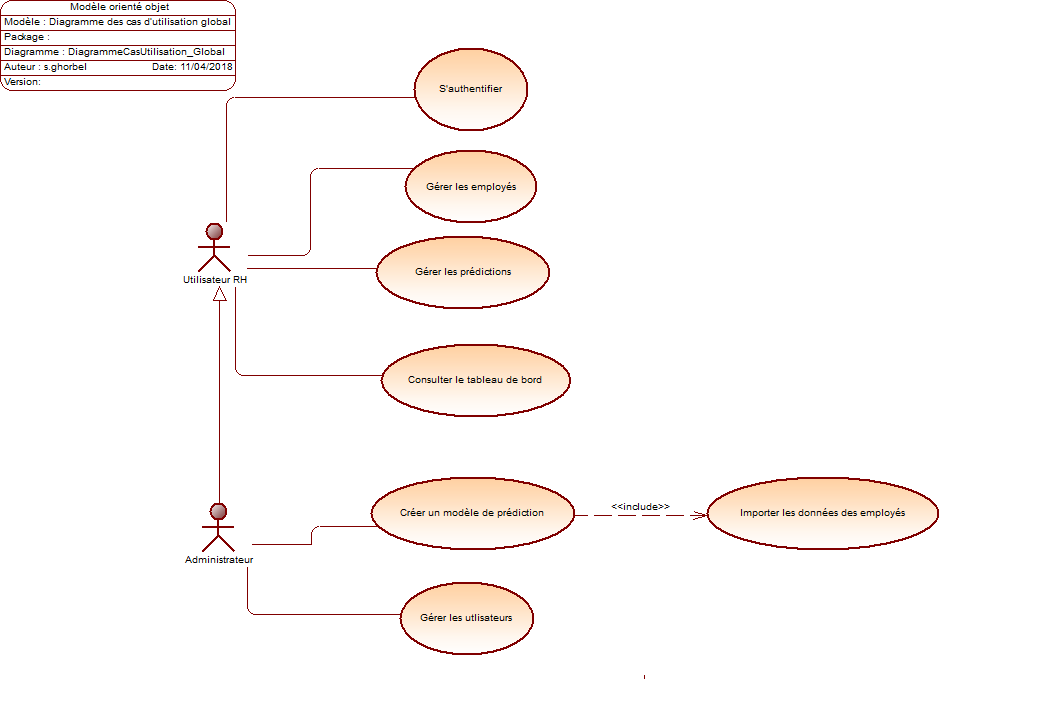
\includegraphics[width=1\linewidth]{img/usecaseglobal_final4.png}}
\fcolorbox{brown}{white}{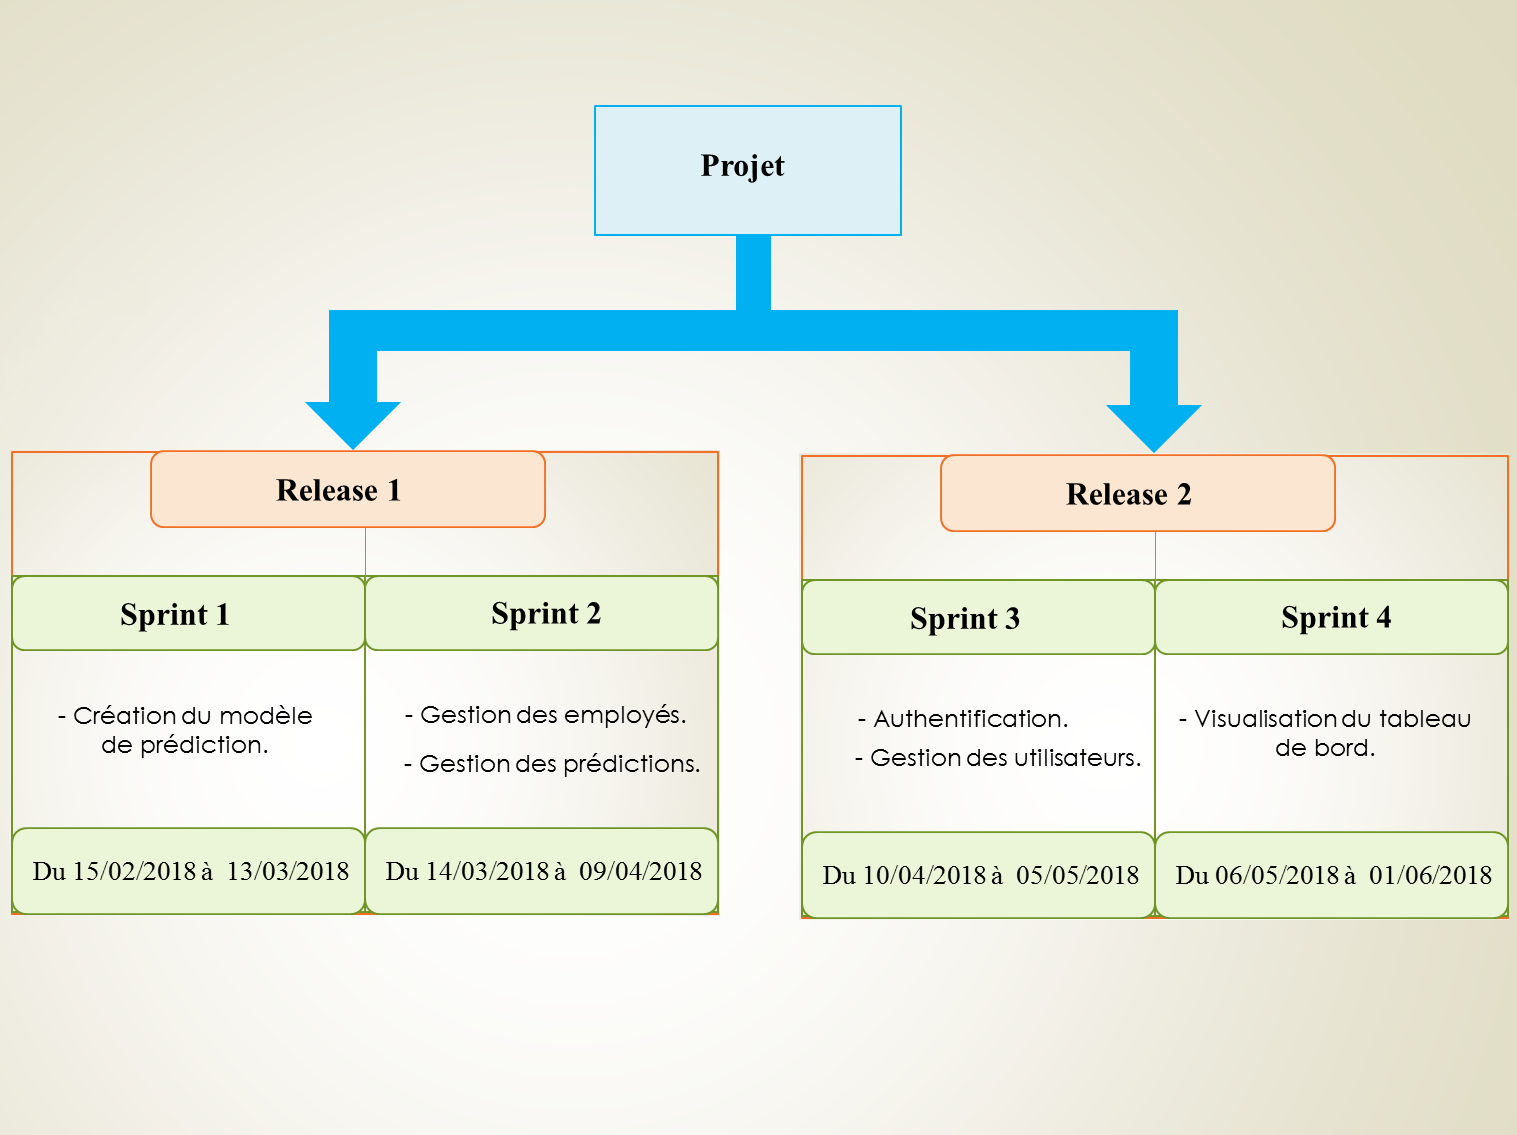
\includegraphics[width=1\linewidth]{img/plannification_sprints_final.png}}
\caption{Planification des sprints}
\label{fig:Planification_des_sprints}
\end{figure}

\section*{Conclusion}
À travers ce chapitre, les différents besoins fonctionnels et non fonctionnels du projet ont été spécifiés. Ils étaient, également, modélisés, en élaborant les diagrammes de cas d’utilisation correspondants par recours au langage de modélisation UML.\\
Le chapitre suivant, intitulé initialisation du projet, sera consacré à la définition de notre environnement de développement et les technologies utilisées.

    
   